\begin{figure}[H]
  \centering
    \def\svgwidth{250pt}
    \begingroup
  \makeatletter
  \providecommand\color[2][]{%
    \errmessage{(Inkscape) Color is used for the text in Inkscape, but the package 'color.sty' is not loaded}
    \renewcommand\color[2][]{}%
  }
  \providecommand\transparent[1]{%
    \errmessage{(Inkscape) Transparency is used (non-zero) for the text in Inkscape, but the package 'transparent.sty' is not loaded}
    \renewcommand\transparent[1]{}%
  }
  \providecommand\rotatebox[2]{#2}
  \ifx\svgwidth\undefined
    \setlength{\unitlength}{184.975pt}
  \else
    \setlength{\unitlength}{\svgwidth}
  \fi
  \global\let\svgwidth\undefined
  \makeatother
  \begin{picture}(1,0.22099066)%
    \put(0,0){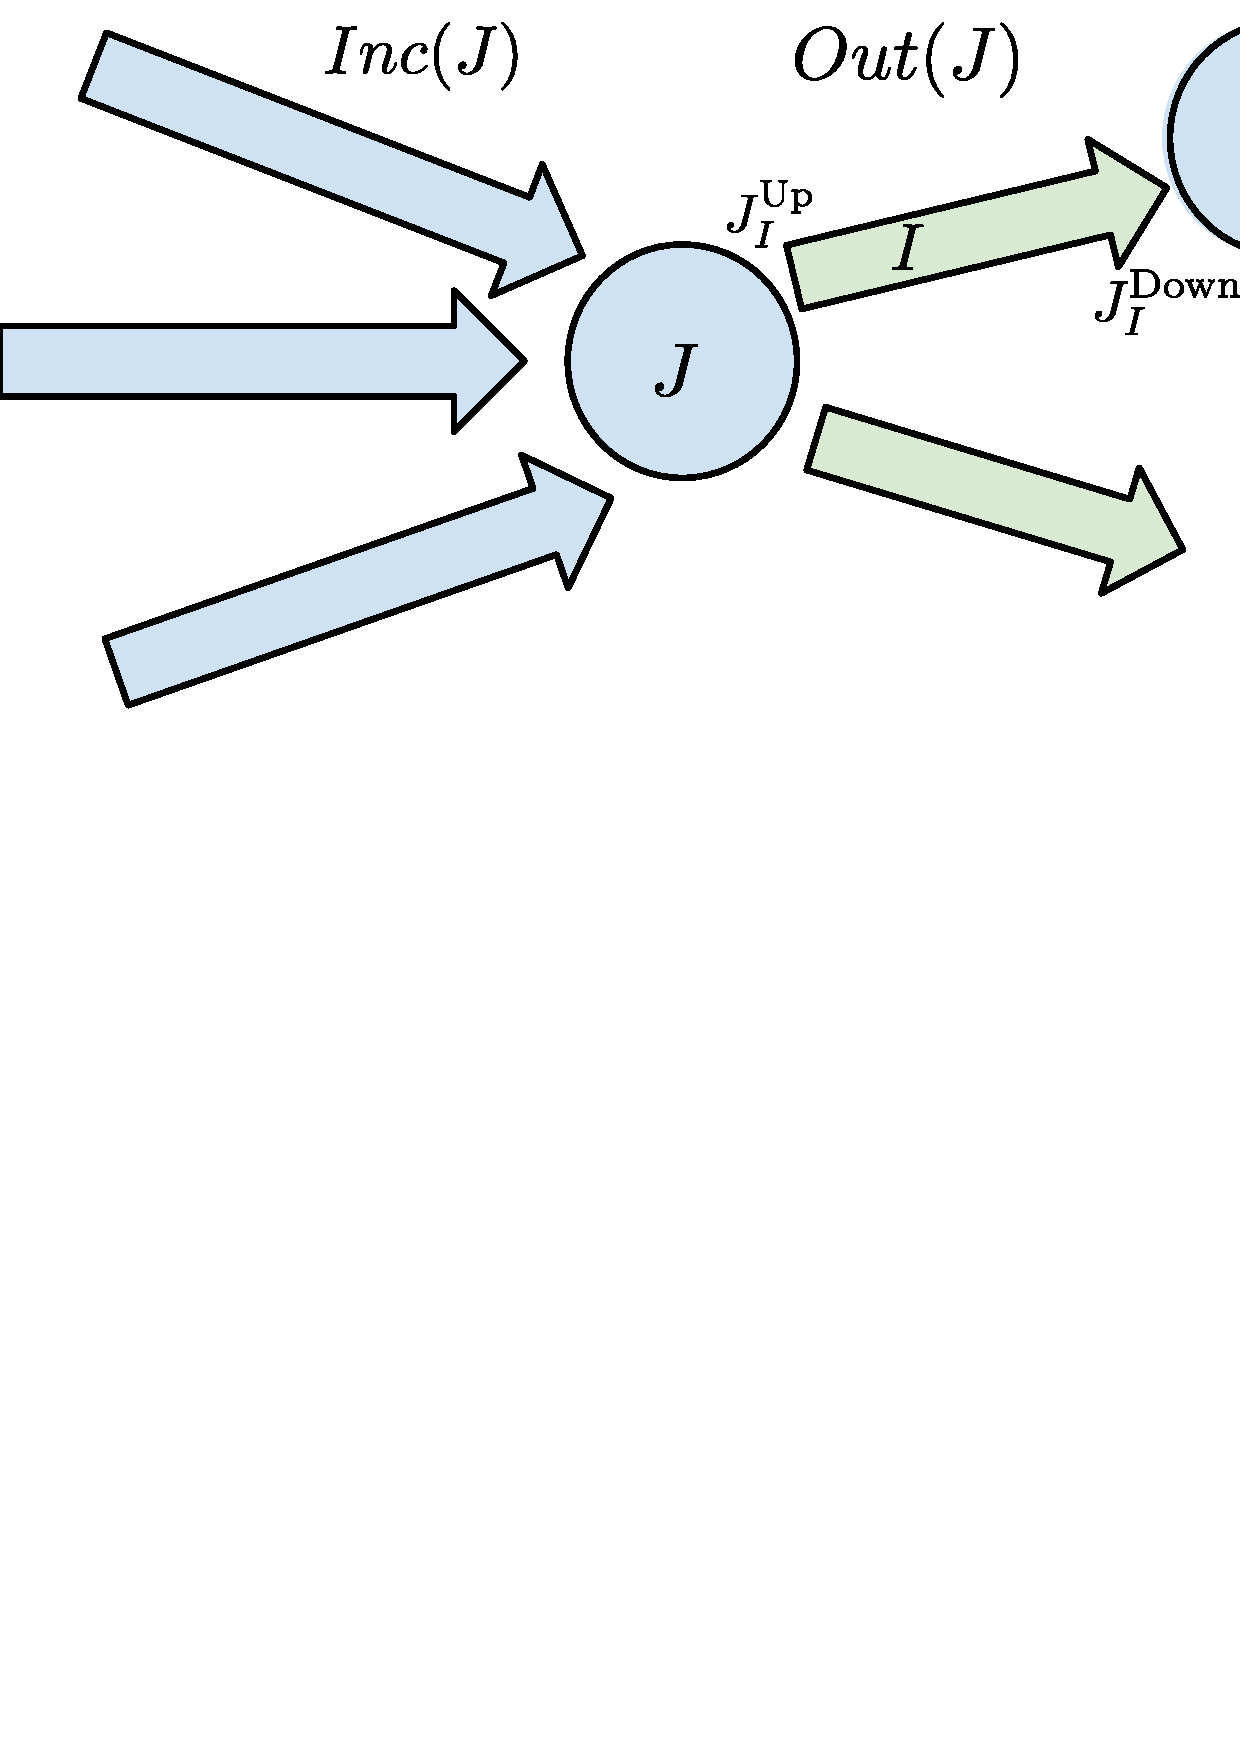
\includegraphics[width=\unitlength]{junction.pdf}}%
    \put(0.50027987,0.16889077){\color[rgb]{0,0,0}\makebox(0,0)[lt]{\begin{minipage}{0.15346451\unitlength}\raggedright $J$\end{minipage}}}%
    \put(0.07871597,0.20074472){\color[rgb]{0,0,0}\makebox(0,0)[lt]{\begin{minipage}{0.3418073\unitlength}\raggedright $I_1$\end{minipage}}}%
    \put(0.89257393,0.20074472){\color[rgb]{0,0,0}\makebox(0,0)[lt]{\begin{minipage}{0.23368458\unitlength}\raggedright $I_2$\end{minipage}}}%
    \put(0.13800905,0.04032891){\color[rgb]{0,0,0}\makebox(0,0)[lt]{\begin{minipage}{0.29995334\unitlength}\raggedright $O_1$\end{minipage}}}%
    \put(0.81791571,0.04032891){\color[rgb]{0,0,0}\makebox(0,0)[lt]{\begin{minipage}{0.25112374\unitlength}\raggedright $O_2$\end{minipage}}}%
  \end{picture}%
	\endgroup
  	\caption{Junction in the network}
	\label{fig:junction}
\end{figure}


\begin{figure}[H]
  \centering
    \def\svgwidth{250pt}
    \begingroup
  \makeatletter
  \providecommand\color[2][]{%
    \errmessage{(Inkscape) Color is used for the text in Inkscape, but the package 'color.sty' is not loaded}
    \renewcommand\color[2][]{}%
  }
  \providecommand\transparent[1]{%
    \errmessage{(Inkscape) Transparency is used (non-zero) for the text in Inkscape, but the package 'transparent.sty' is not loaded}
    \renewcommand\transparent[1]{}%
  }
  \providecommand\rotatebox[2]{#2}
  \ifx\svgwidth\undefined
    \setlength{\unitlength}{208.30859375pt}
  \else
    \setlength{\unitlength}{\svgwidth}
  \fi
  \global\let\svgwidth\undefined
  \makeatother
  \begin{picture}(1,0.5924706)%
    \put(0,0){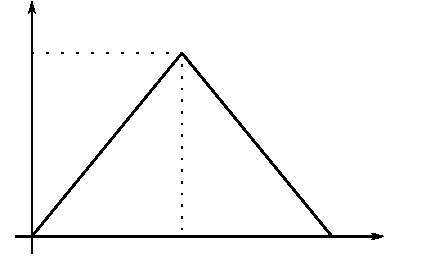
\includegraphics[width=\unitlength]{flux.pdf}}%
    \put(-0.02516719,0.58497148){\color[rgb]{0,0,0}\makebox(0,0)[lt]{\begin{minipage}{0.17546911\unitlength}\raggedright $f(\rho)$\end{minipage}}}%
    \put(0.8717455,0.03536558){\color[rgb]{0,0,0}\makebox(0,0)[lt]{\begin{minipage}{0.25492683\unitlength}\raggedright $\rho$\end{minipage}}}%
    \put(0.7264574,0.03536558){\color[rgb]{0,0,0}\makebox(0,0)[lt]{\begin{minipage}{0.32047942\unitlength}\raggedright $\rho_{max}$\end{minipage}}}%
    \put(-0.02516719,0.50824099){\color[rgb]{0,0,0}\makebox(0,0)[lt]{\begin{minipage}{0.25227822\unitlength}\raggedright $f^{max}$\end{minipage}}}%
    \put(0.38091568,0.03536558){\color[rgb]{0,0,0}\makebox(0,0)[lt]{\begin{minipage}{0.57601045\unitlength}\raggedright $\rho^{cr}$\end{minipage}}}%
  \end{picture}%
	\endgroup
    \caption{Fundamental diagram}
	\label{fig:FDiag}
\end{figure}